\documentclass[xcolor=pdftex,dvipsnames,table,mathserif,aspectratio=169]{beamer}
\usetheme{metropolis}

\usepackage[english]{babel}
\usepackage{pgf,pgfarrows,pgfnodes,pgfautomata,pgfheaps}
\usepackage{amsmath,amssymb,setspace,centernot}
\usepackage[latin1]{inputenc}
\usepackage[T1]{fontenc}
\usepackage{relsize}
\usepackage{pdfpages}
\usepackage[absolute,overlay]{textpos} 

\newenvironment{reference}[2]{% 
  \begin{textblock*}{\textwidth}(#1,#2) 
      \footnotesize\it\bgroup\color{red!50!black}}{\egroup\end{textblock*}} 

\DeclareMathSizes{10}{10}{6}{6} 
\AtBeginSection[]{
  \begin{frame}
  \vfill
  \centering
  \begin{beamercolorbox}[sep=8pt,center,shadow=true,rounded=true]{title}
    \usebeamerfont{title}\insertsectionhead\par%
  \end{beamercolorbox}
  \vfill
  \end{frame}
}


\DeclareMathOperator*{\argmax}{arg\,max}
\DeclareMathOperator*{\argmin}{arg\,min}

\newcommand{\norm}[1]{\left\lVert#1\right\rVert}
\newcommand{\X}{\mathtt{X}}
\newcommand{\Y}{\mathtt{Y}}

%\newcommand{\R}{\mathbb{R}}
%\newcommand{\E}{\mathbb{E}}
%\newcommand{\V}{\mathbb{V}}
\newcommand{\p}{\mathbb{P}}
\newcommand*\df{\mathop{}\!\mathrm{d}}
\newcommand{\del}{\partial}

\begin{document}
\title{Extensions and Variants}
\author{Chris Conlon}
\institute{Grad IO}
\date{\today}

\frame{\titlepage}


\begin{frame}
\frametitle{BLP Extensions: Demographics}
\begin{itemize}
\item It is helpful to allow for interactions with consumer demographics (such as income).
\item A few ways to do this:
\begin{itemize}
\item You could just use cross sectional variation in $s_{jt}$ and $\overline{y}_t$ (mean or median income).
\item Better: Divide up your data into additional ``markets'' by demographics: do you observe $\mathfrak{s}_{jt}$ at this level? [May not be possible!]
\item Better: Draw $y_{it}$ from a geographic specific income distribution. Draw $\nu_i$ from a general distribution of unobserved heterogeneity.
\end{itemize}
\item Ex: Nevo (2000) Cereal demand sampled individual level $D_i$ from geographic specific CPS data
\item Joint distribution of income, income-squared, age, child at home.
\begin{align*}
\beta_i = \overline{\beta} + \Pi D_i + \sigma \nu_i
\end{align*}
\end{itemize}
\end{frame}

\begin{frame}
\frametitle{BLP Extensions: Panel Data}
\begin{itemize}
\item with enough observations on the same product it is possible to include fixed effects
\begin{eqnarray*}
\delta_{jt}(\widetilde{\theta}_2) = x_{jt} \beta - \alpha p_{jt} + \underbrace{\xi_{jt}}_{\xi_{j} + \xi_t + \Delta \xi_{jt}}
\end{eqnarray*}
\item What does $\xi_{j}$ mean in this context?
\item What would $\xi_t$ mean in this context?
\item $\Delta \xi_{jt}$ is now the structural error term, this changes our identification strategy a little.
\item We need instruments that change \alert{within product and across market}.
\end{itemize}
\end{frame}

\begin{frame}
\frametitle{Extensions: Micro Data (Petrin 2002), (microBLP 2004)}
Suppose we had additional data on behavior of individuals (in addition to aggregate market shares).
\begin{itemize}
\item Examples:
\begin{itemize}
\item For some customers have answer to ``Which car would you have purchased if the car you bought was not available?''
\item Demographic data on purchasers of a single brand.
\item Full individual demographic and choice data.
\end{itemize}
\end{itemize}
\end{frame}

\begin{frame}
\frametitle{Extensions: Micro Data: Nielsen Panelists}
Nielsen data surveys panelists on everything they buy with a UPC code including what store they purchased from.
\begin{itemize}
\item Also tracks household characteristics (Race, Income, Education, HH Size, etc.)
\item Can calculate covariance of characteristics (such as price) with demographics (income, education, etc.) \alert{conditional on purchase}
\item Can calculate purchase probability conditional on demographics: Did you buy any yogurt this trip, week, month, year?
\end{itemize}
Should we use these as individual data? Or Aggregate data from scanner data with additional moments?
\end{frame}

\begin{frame} \frametitle{Extensions: Micro Data (Petrin 2002), (microBLP 2004)}
\begin{itemize}
\item Previously we had moment conditions from orthogonality of structural error $(\xi)$ and $(X,Z)$ in order to form our GMM objective.
\begin{eqnarray*}
E[\xi_{jt} | z_{jt}]=0 \rightarrow E[\xi_{jt}' Z_{jt}]=0
\end{eqnarray*}
\item We can incorporate additional information using ``micro-moments'' or additional moment conditions to match the micro data.
\begin{itemize}
\item $Pr(\mbox{ i buys j } | y_i \in [0,\$20K])= c_1$ or  $Cov(d_i, s_{ijt}) = c_2$
\item Construct an additional error term $\zeta_1,\zeta_2$ and interact that with instruments to form additional moment conditions.
\item Econometrics get tricky when we have a different number of observations for $E[\zeta'  Z_m]=0$ and  $E[\xi'  Z_d]=0$.
\begin{itemize}
\item May not be able to get covariance of moments taken over different sets of observations!
\item People often assume optimal weight matrices are block diagonal.
\end{itemize}
\end{itemize}
\end{itemize}
\end{frame}




\begin{frame}
\frametitle{Alternative: Vertical Model (Bresnahan 1987)}
\footnotesize
\begin{itemize}
\item Imagine everyone agreed on the quality of the products offered for sale.
\item The only thing people disagree on is willingness to pay for quality
\begin{eqnarray*}
U_{ij} = \overline{u} + \delta_j - \alpha_i p_j
\end{eqnarray*}
\item How do we estimate?
\begin{itemize}
\item Sort goods from $p_1 < p_2  < p_3 \ldots < p_J$.\\
 It must be that $\delta_1 < \delta_2 < \ldots < \delta_J$. Why?
 \item Normalize o.g. to $0$ so that $ 0 > \delta_1 -\alpha_i p_1$ or $\alpha_i > \delta_1 / p_1$.
 \item $s_0 = F(\infty) - F(\frac{\delta_1}{p_1})  = 1 - F(\frac{\delta_1}{p_1}) $ where $F(\cdot)$ is CDF of $\alpha_i$.
 \item In general choose $j$ IFF:
 \begin{eqnarray*}
 \frac{\delta_{j+1} - \delta_j}{p_{j+1} -p_j} < \alpha_i < \frac{\delta_j  - \delta_{j-1}}{p_j - p_{j-1}}\\
 s_j = F\left(\frac{\delta_{j+1} - \delta_j}{p_{j+1} -p_j} \right) - F\left(\frac{\delta_j  - \delta_{j-1}}{p_j - p_{j-1}} \right)
 \end{eqnarray*}
\end{itemize}
\end{itemize}
\end{frame}

\begin{frame}
\frametitle{Alternative: Vertical Model (Bresnahan 1987)}
Estimation
\begin{itemize}
\item Choose parameters $\theta$ of $F(\cdot)$ in order to best match $s_j$.
\begin{itemize}
\item Can do MLE $\arg \max_{\theta} \sum_j -\mathfrak{s}_j \log s_{j}(\theta)$.
\item Can do least squares $\sum_j (\mathfrak{s}_j - s_{j}(\theta) )^2$.
\item Can do IV/GMM if I have an instrument for price.  $\delta_j = x_j \beta + \xi_j$.
\item Extremely easy when $F\sim \exp(\lambda)$.
\end{itemize}
\item What about elasticities?
\begin{itemize}
\item When I change the price of $j$ it can only affect $(s_{j-1},s_j, s_{j+1})$.
\item We have set all of the other cross-price elasticities to be zero.
\item If a luxury car and a truck have similar prices, this can create strange substitution patterns.
\end{itemize}
\end{itemize}
\end{frame}

\begin{frame} \frametitle{Pure Characteristics Model: Berry Pakes (2001/2007)}
\footnotesize
\begin{eqnarray*}
u_{ij} = \delta_j + \sum_k \nu_{ik} x_{jk} + \xi_{j} + \underbrace{\sigma_i \varepsilon_{ij}}_{\rightarrow 0}
\end{eqnarray*}
\begin{itemize}
\item Can think of this like random coefficients model where we take the variance of $\epsilon$ to zero.
\item Can think of this a vertical model, with vertical tastes over several characteristics.
\begin{itemize}
\item PCs: everyone prefers more Mhz, more RAM, and more storage but differ in WTP.
\item Possible that there is no PC specific $\varepsilon$.
\end{itemize}
\item Advantages
\begin{itemize}
\item Logit error means there is always some substitution to all other goods. 
\item Reality may be you only compete with a small number of competitors.
\item Allows for \alert{crowding} in the product space.
\end{itemize}
\item Disadvantage: no closed form for $s_j$, so estimation is extremely difficult.
\item Minjae Song (Homotopy) and Che-Lin Su (MPCC) have made progress using two different approaches.
\end{itemize}
\end{frame}

%
%\begin{frame}{Differentiation Instruments: Gandhi Houde (2016)}
%\begin{center}
%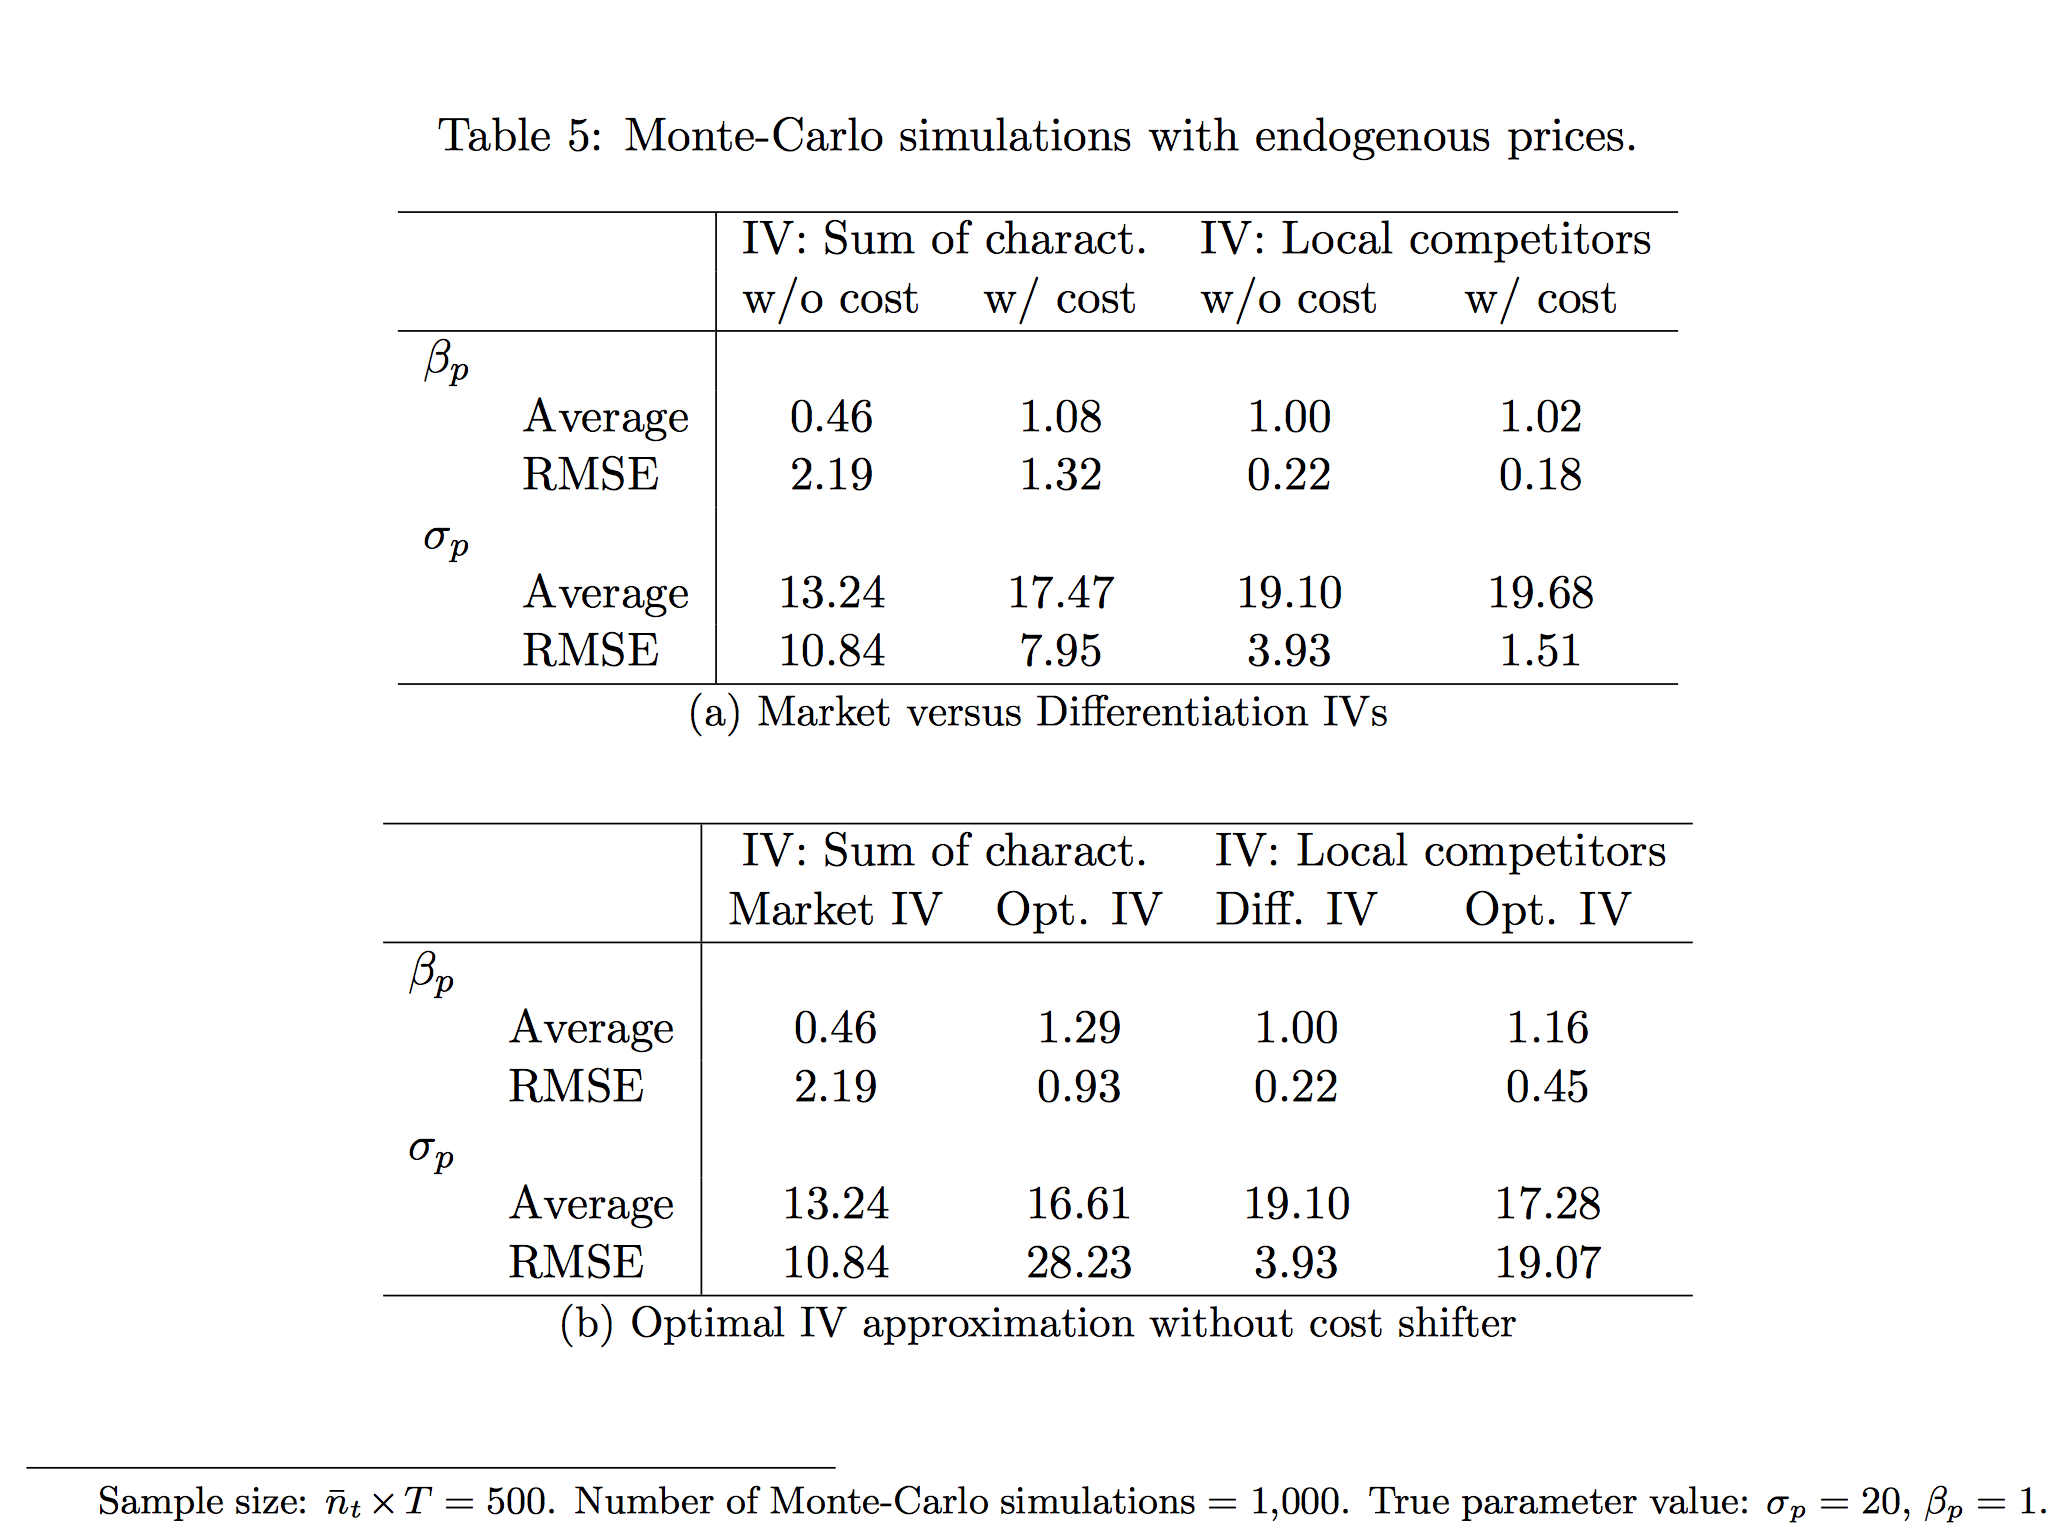
\includegraphics[width=3.8in]{resources/d_iv2.png}
%\end{center}
%\end{frame}
%



%
%\begin{frame} \frametitle{Extensions: Supply Moments}
%\begin{itemize}
%\item We can also impose the Bertrand FOC as a set of additional moments.
%\item First parametrize marginal cost
%\begin{eqnarray*}
%\ln mc_{jt} = \gamma_1 x_{jt} + \gamma_2 w_{jt} + \omega_{jt}
%\end{eqnarray*}
%\item helpful to constrain MC to be positive always.
%\item Note that for any vector of prices $p$ and demand parameters $\theta$ we can recover a unique vector of marginal costs (by solving the system of linear equations).
%\item Imposing the supply side only helps if we have information about the marginal costs / production function that we would like to impose
%\item Imposing these restrictions is helpful in constraining markups (so that implied MC are always positive, etc.).
%\item Misspecified functional forms for costs can cause problems!
%\end{itemize}
%\end{frame}





\end{document}